\documentclass[aspectratio=169]{beamer}
\usepackage[utf8]{inputenc}
\usepackage{amsmath, amssymb}
\usepackage{tikz}

\title{}
\author{{\LARGE Suzie Brown}}
\date{30 October 2018} 

\begin{document}

\begin{frame}
\maketitle
\end{frame}

\begin{frame}
\begin{tikzpicture}
  \node (img1a) at (0,0) {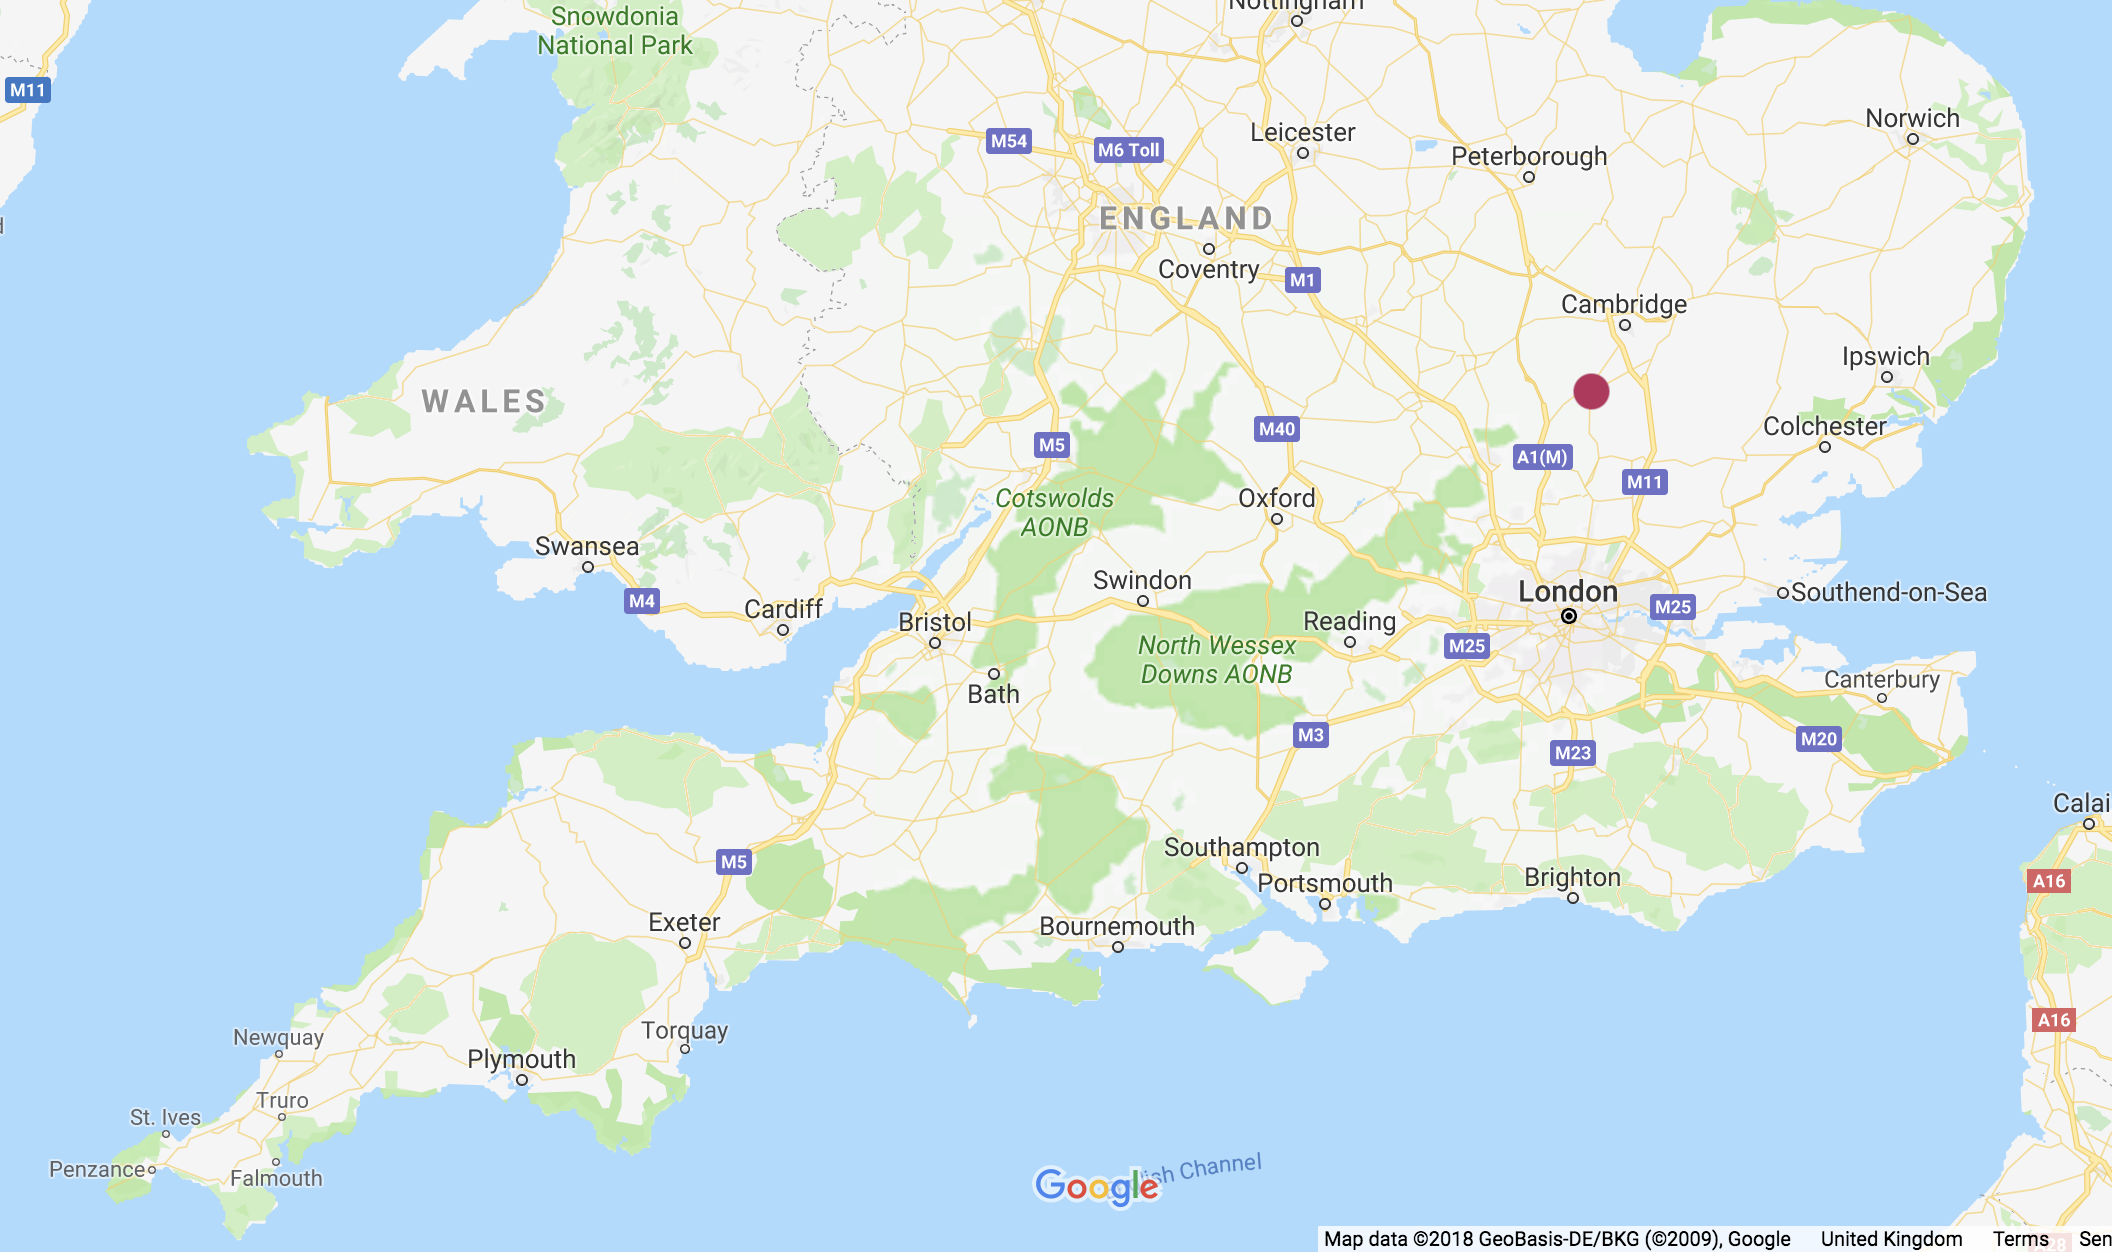
\includegraphics[width=\textwidth]{map1.png}};
  \node (img1b) at (-3.3,-1.5) {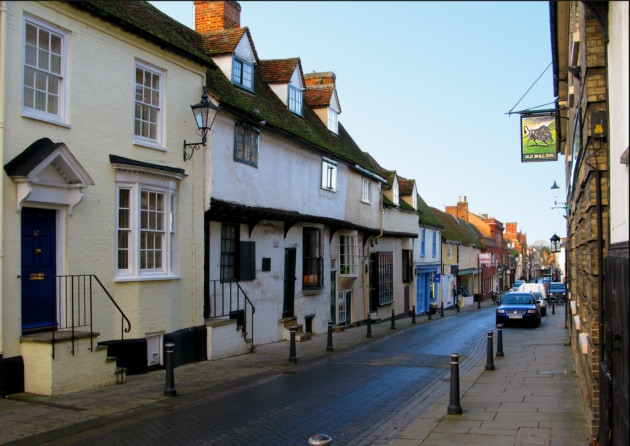
\includegraphics[height=5cm]{royston.jpg}};
\end{tikzpicture}
\end{frame}

\begin{frame}
\begin{tikzpicture}
  \node (img1a) at (0,0) {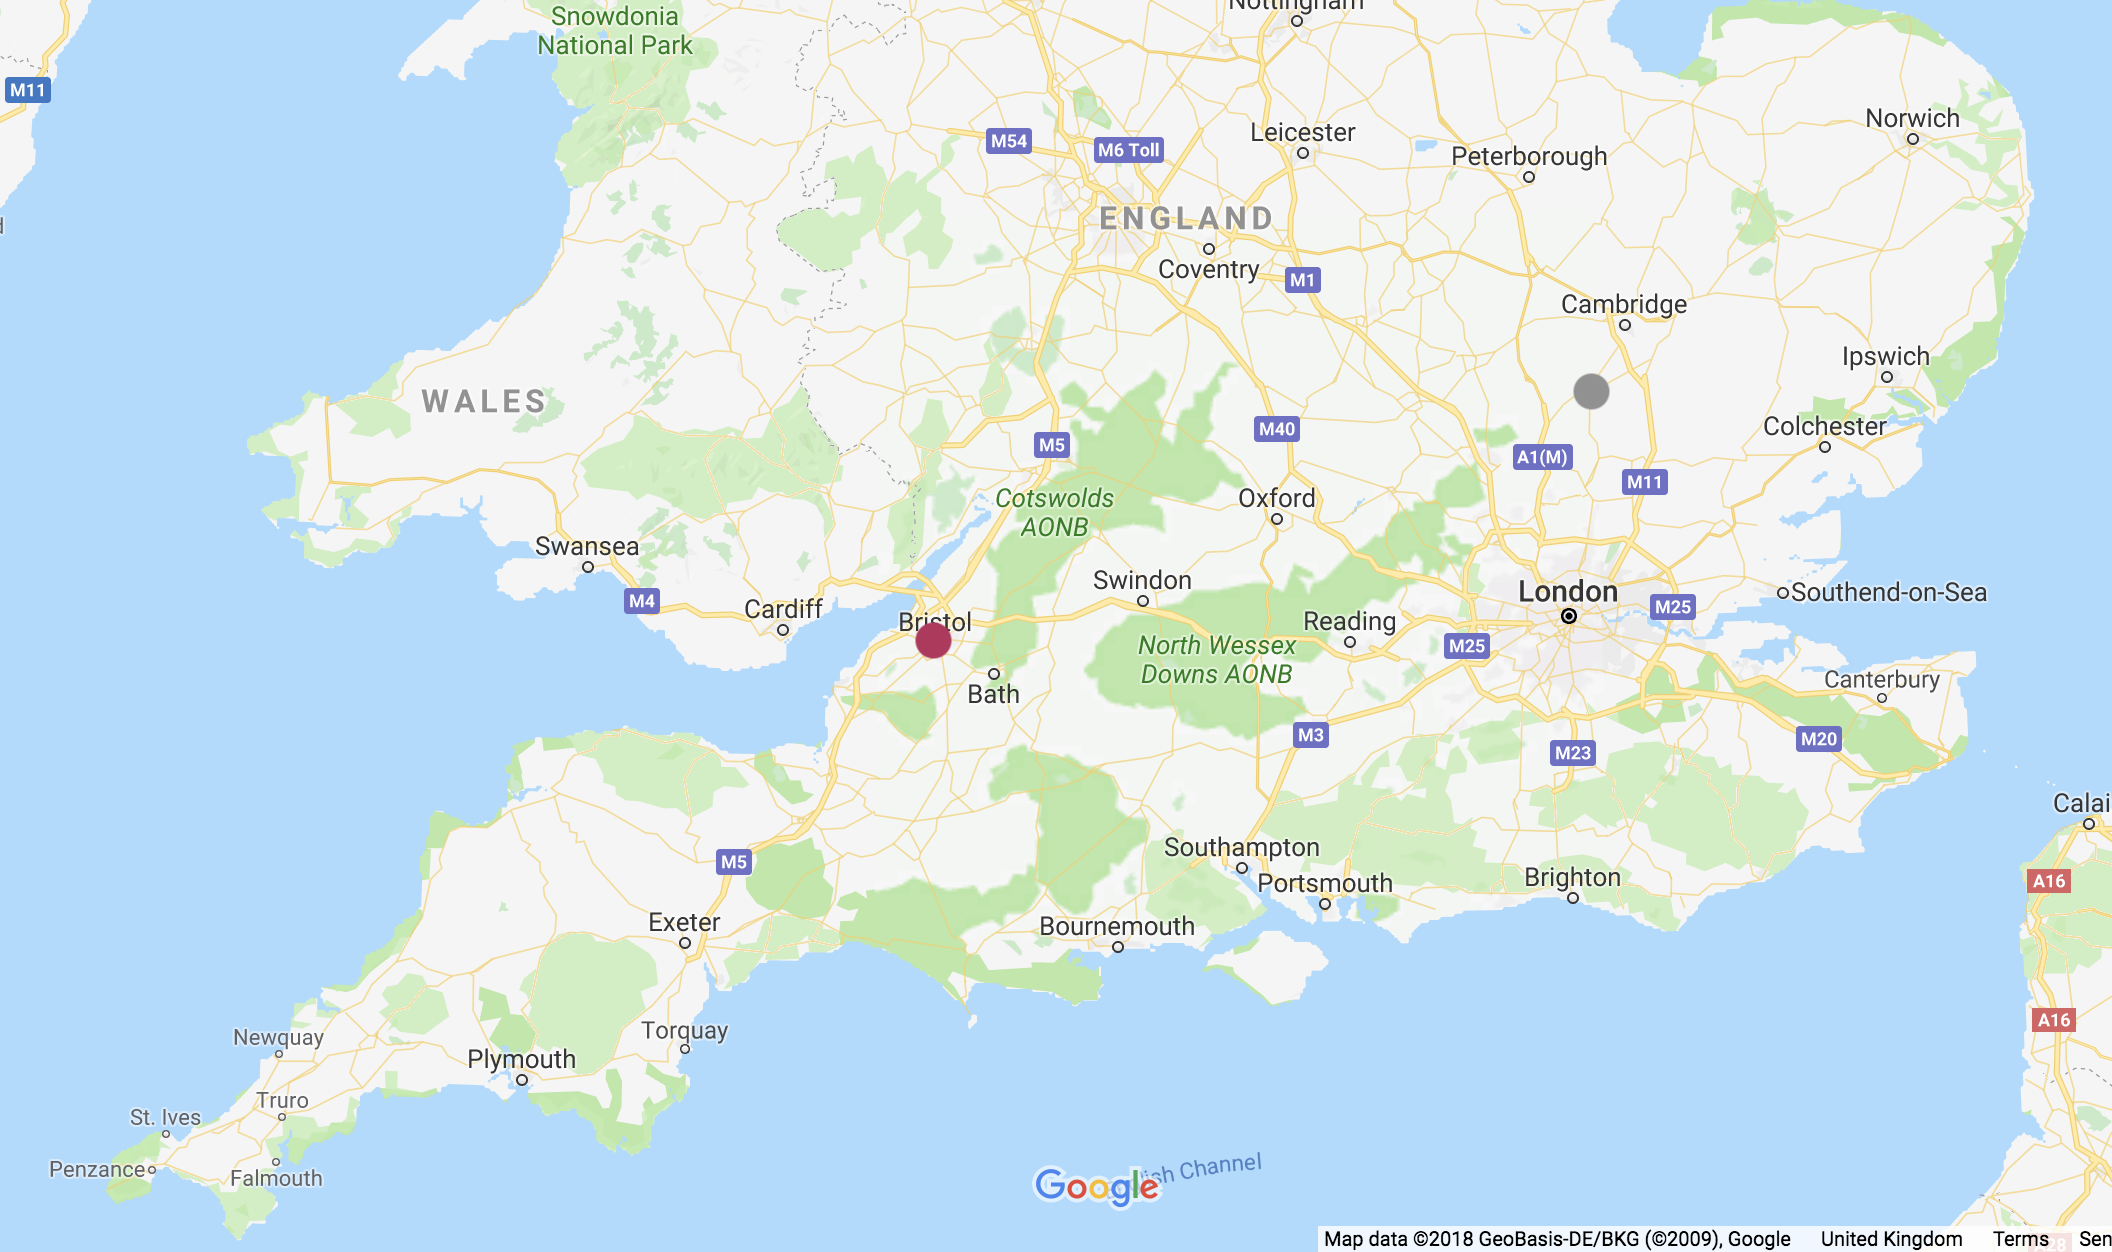
\includegraphics[width=\textwidth]{map2.png}};
  \node (img1b) at (3.4,-1.6) {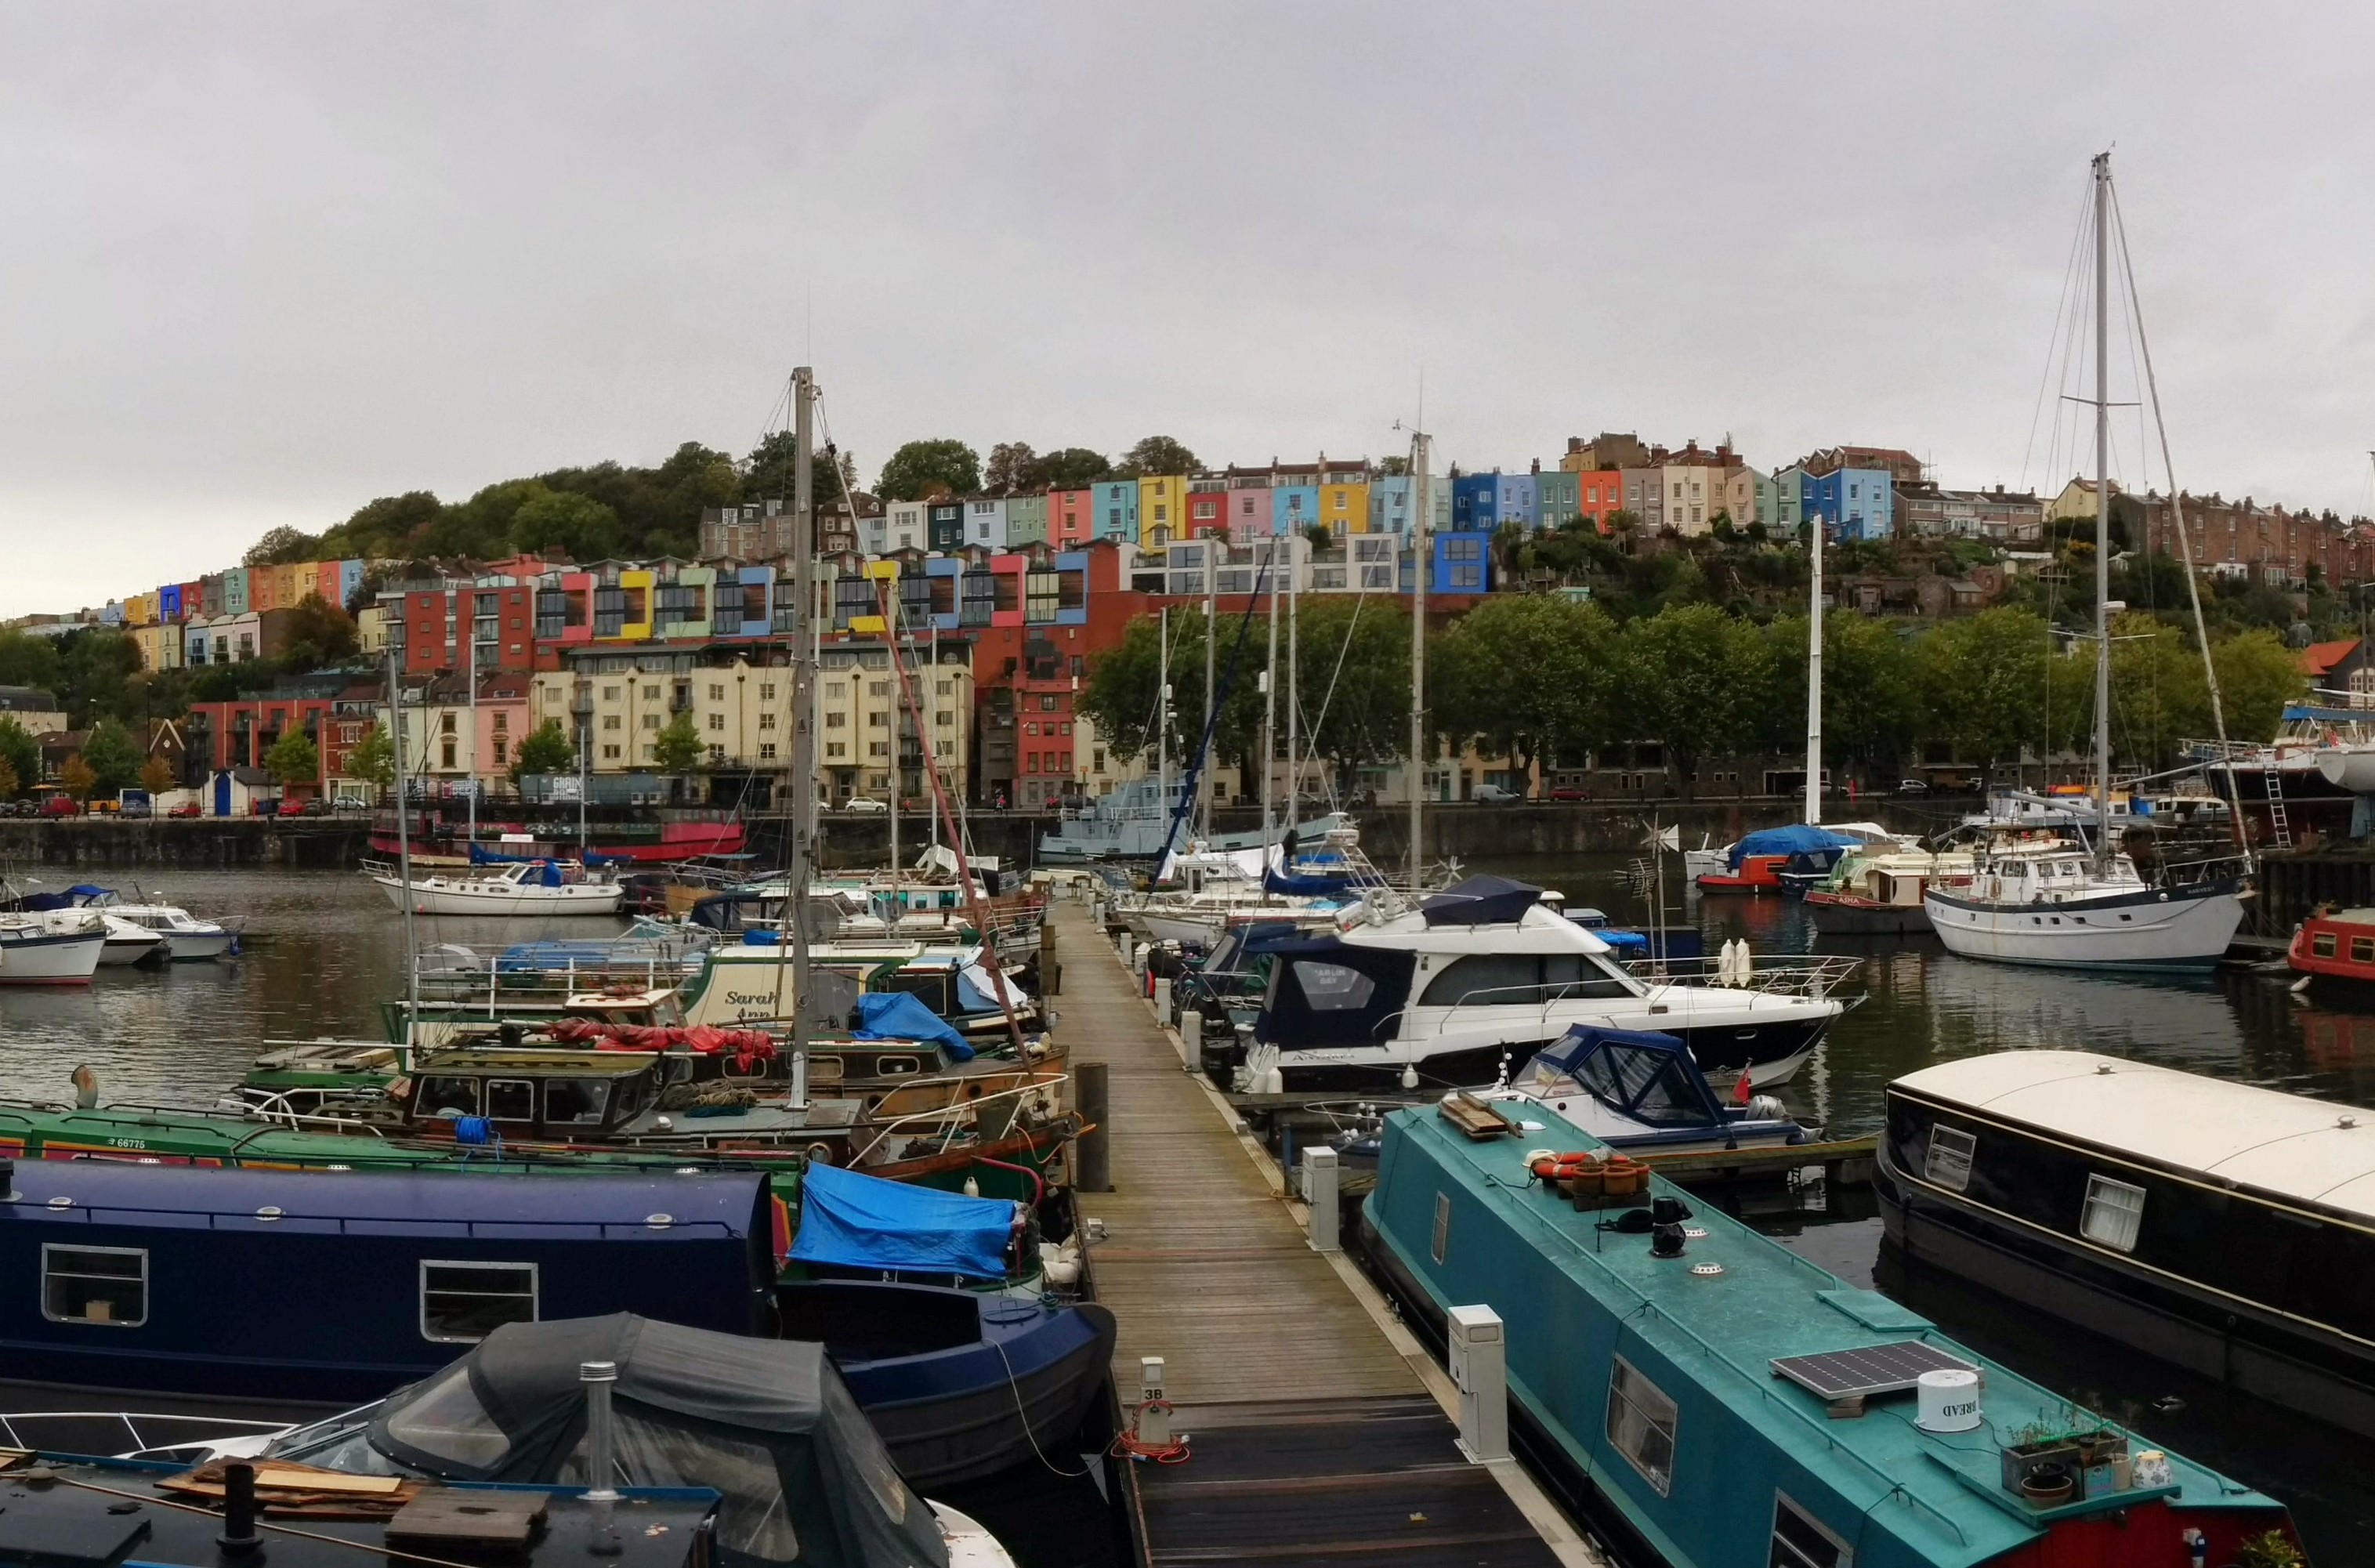
\includegraphics[height=4.5cm]{bristol.jpg}};
\end{tikzpicture}
\end{frame}

\begin{frame}
\begin{columns}
\begin{column}{0.45\textwidth}
{\LARGE Estimating the probability that a sparse random binary matrix has full rank}\\[10pt]
{\footnotesize Brown, S., Johnson, O. and Tassi, A., 2018. \textbf{Reliability of broadcast communications under sparse random linear network coding.} \textit{IEEE Transactions on Vehicular Technology}, 67(5), pp.4677-4682.}
\end{column}
\begin{column}{0.25\textwidth}
\centering
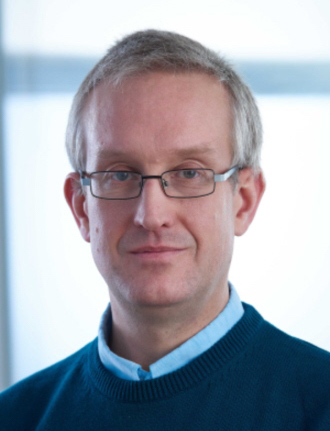
\includegraphics[width=\textwidth]{olly.jpg}\\
Olly Johnson
\end{column}
\begin{column}{0.25\textwidth}
\centering
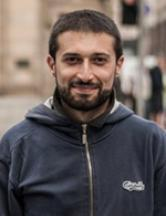
\includegraphics[width=\textwidth]{andrea.jpeg}\\
Andrea Tassi
\end{column}
\end{columns}
\end{frame}

\begin{frame}
\begin{columns}
\begin{column}{0.45\textwidth}
{\LARGE Hamiltonian Monte Carlo:\\ Theory \& Practice}
\end{column}
\begin{column}{0.45\textwidth}
\centering
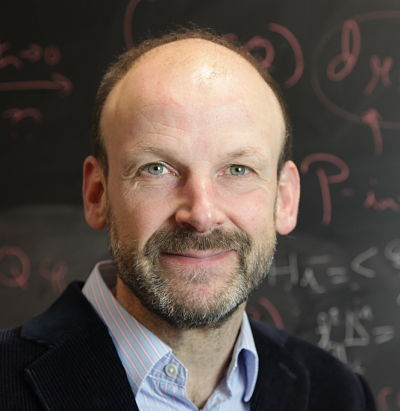
\includegraphics[width=0.6\textwidth]{jonty.jpg}\\
Jonty Rougier
\end{column}
\end{columns}
\end{frame}

\begin{frame}
\begin{tikzpicture}
  \node (img1a) at (0,0) {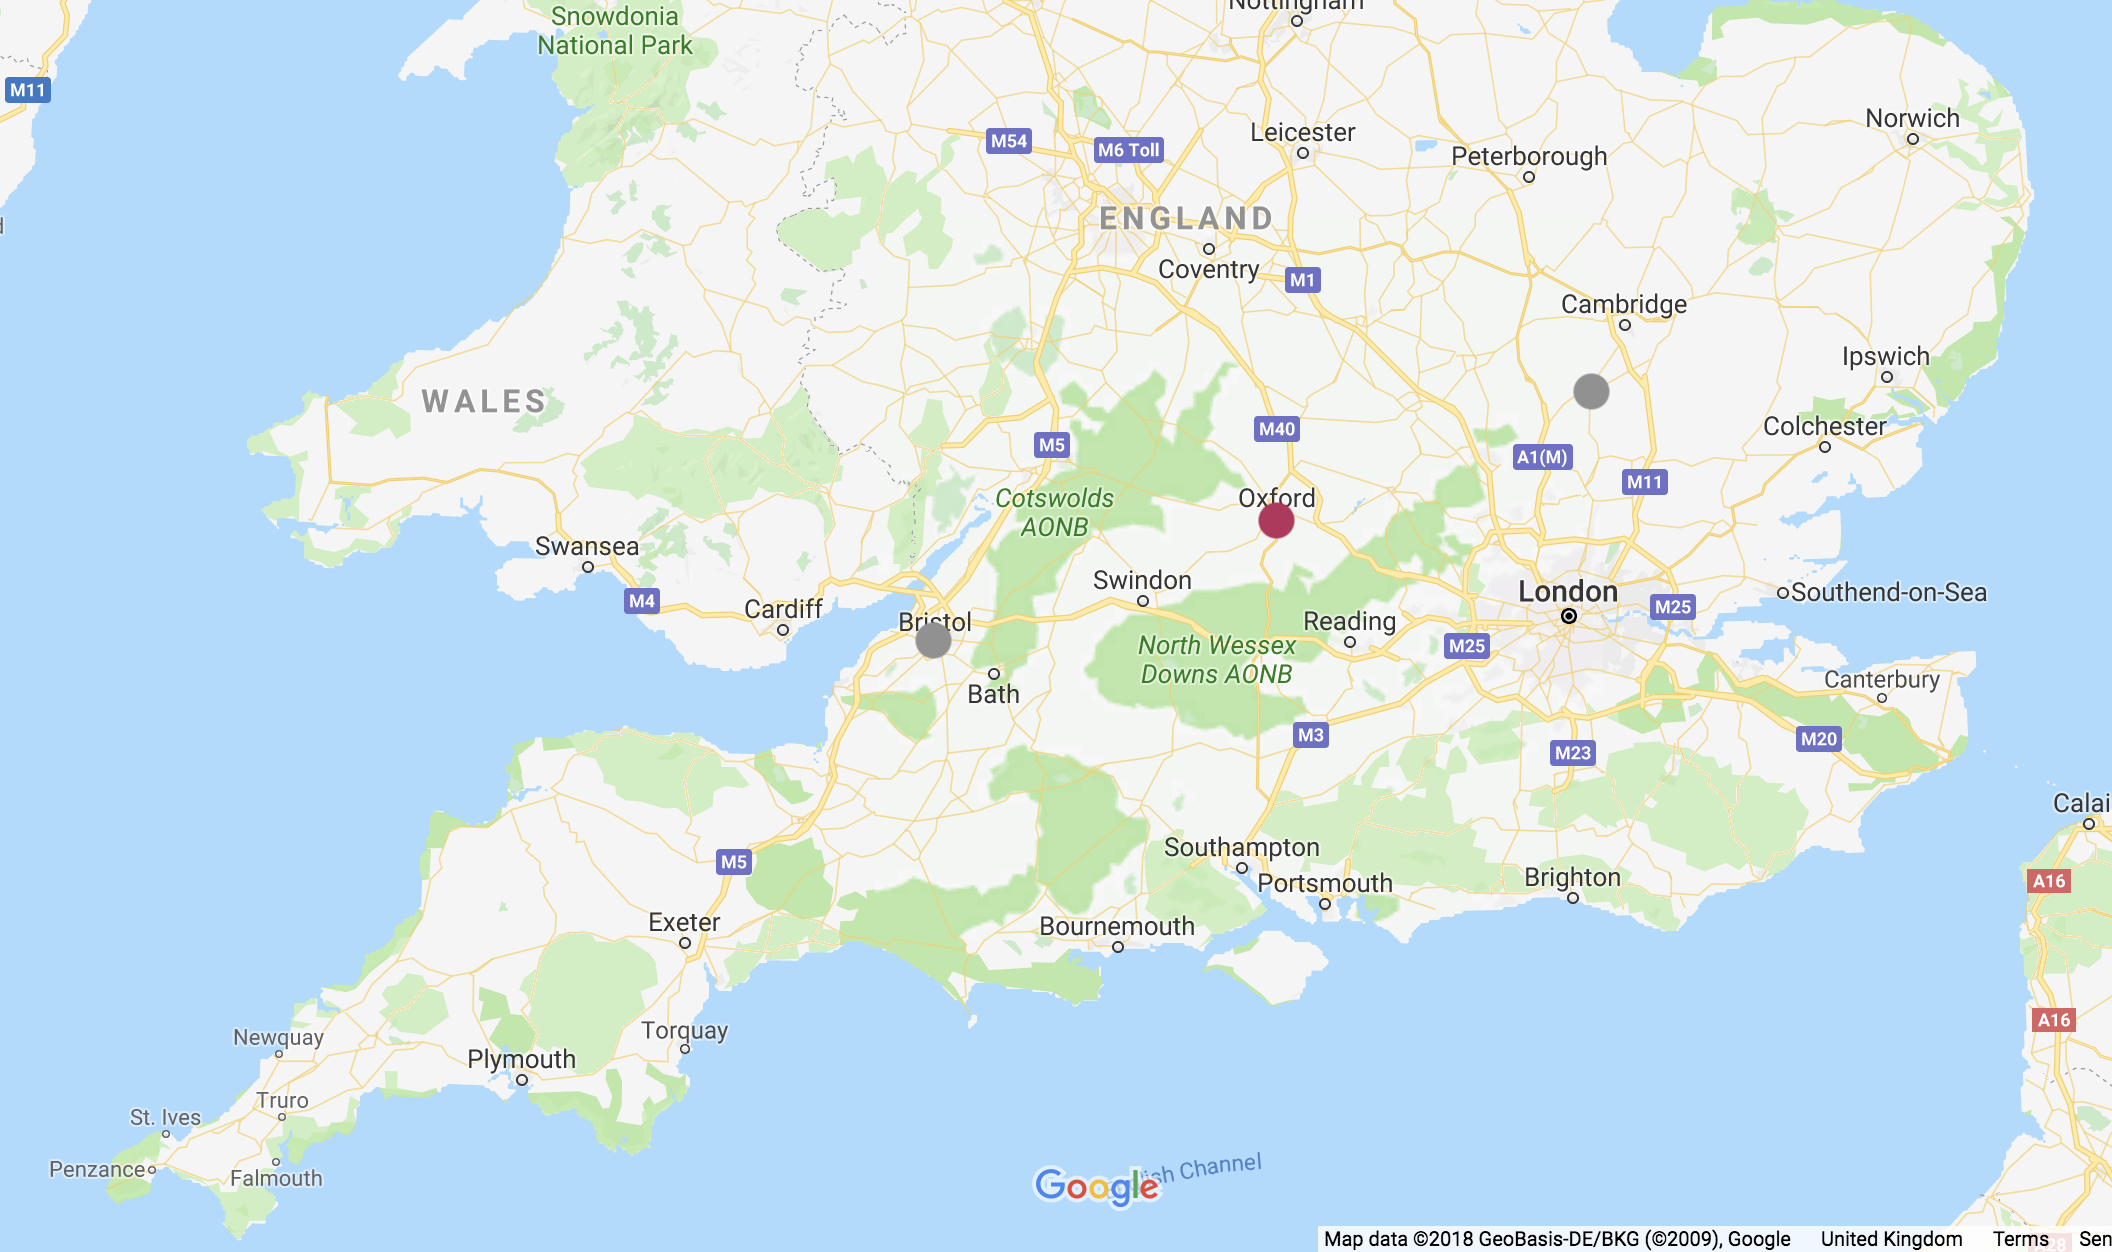
\includegraphics[width=\textwidth]{map3.png}};
  \node (img1b) at (-4.2,-1) {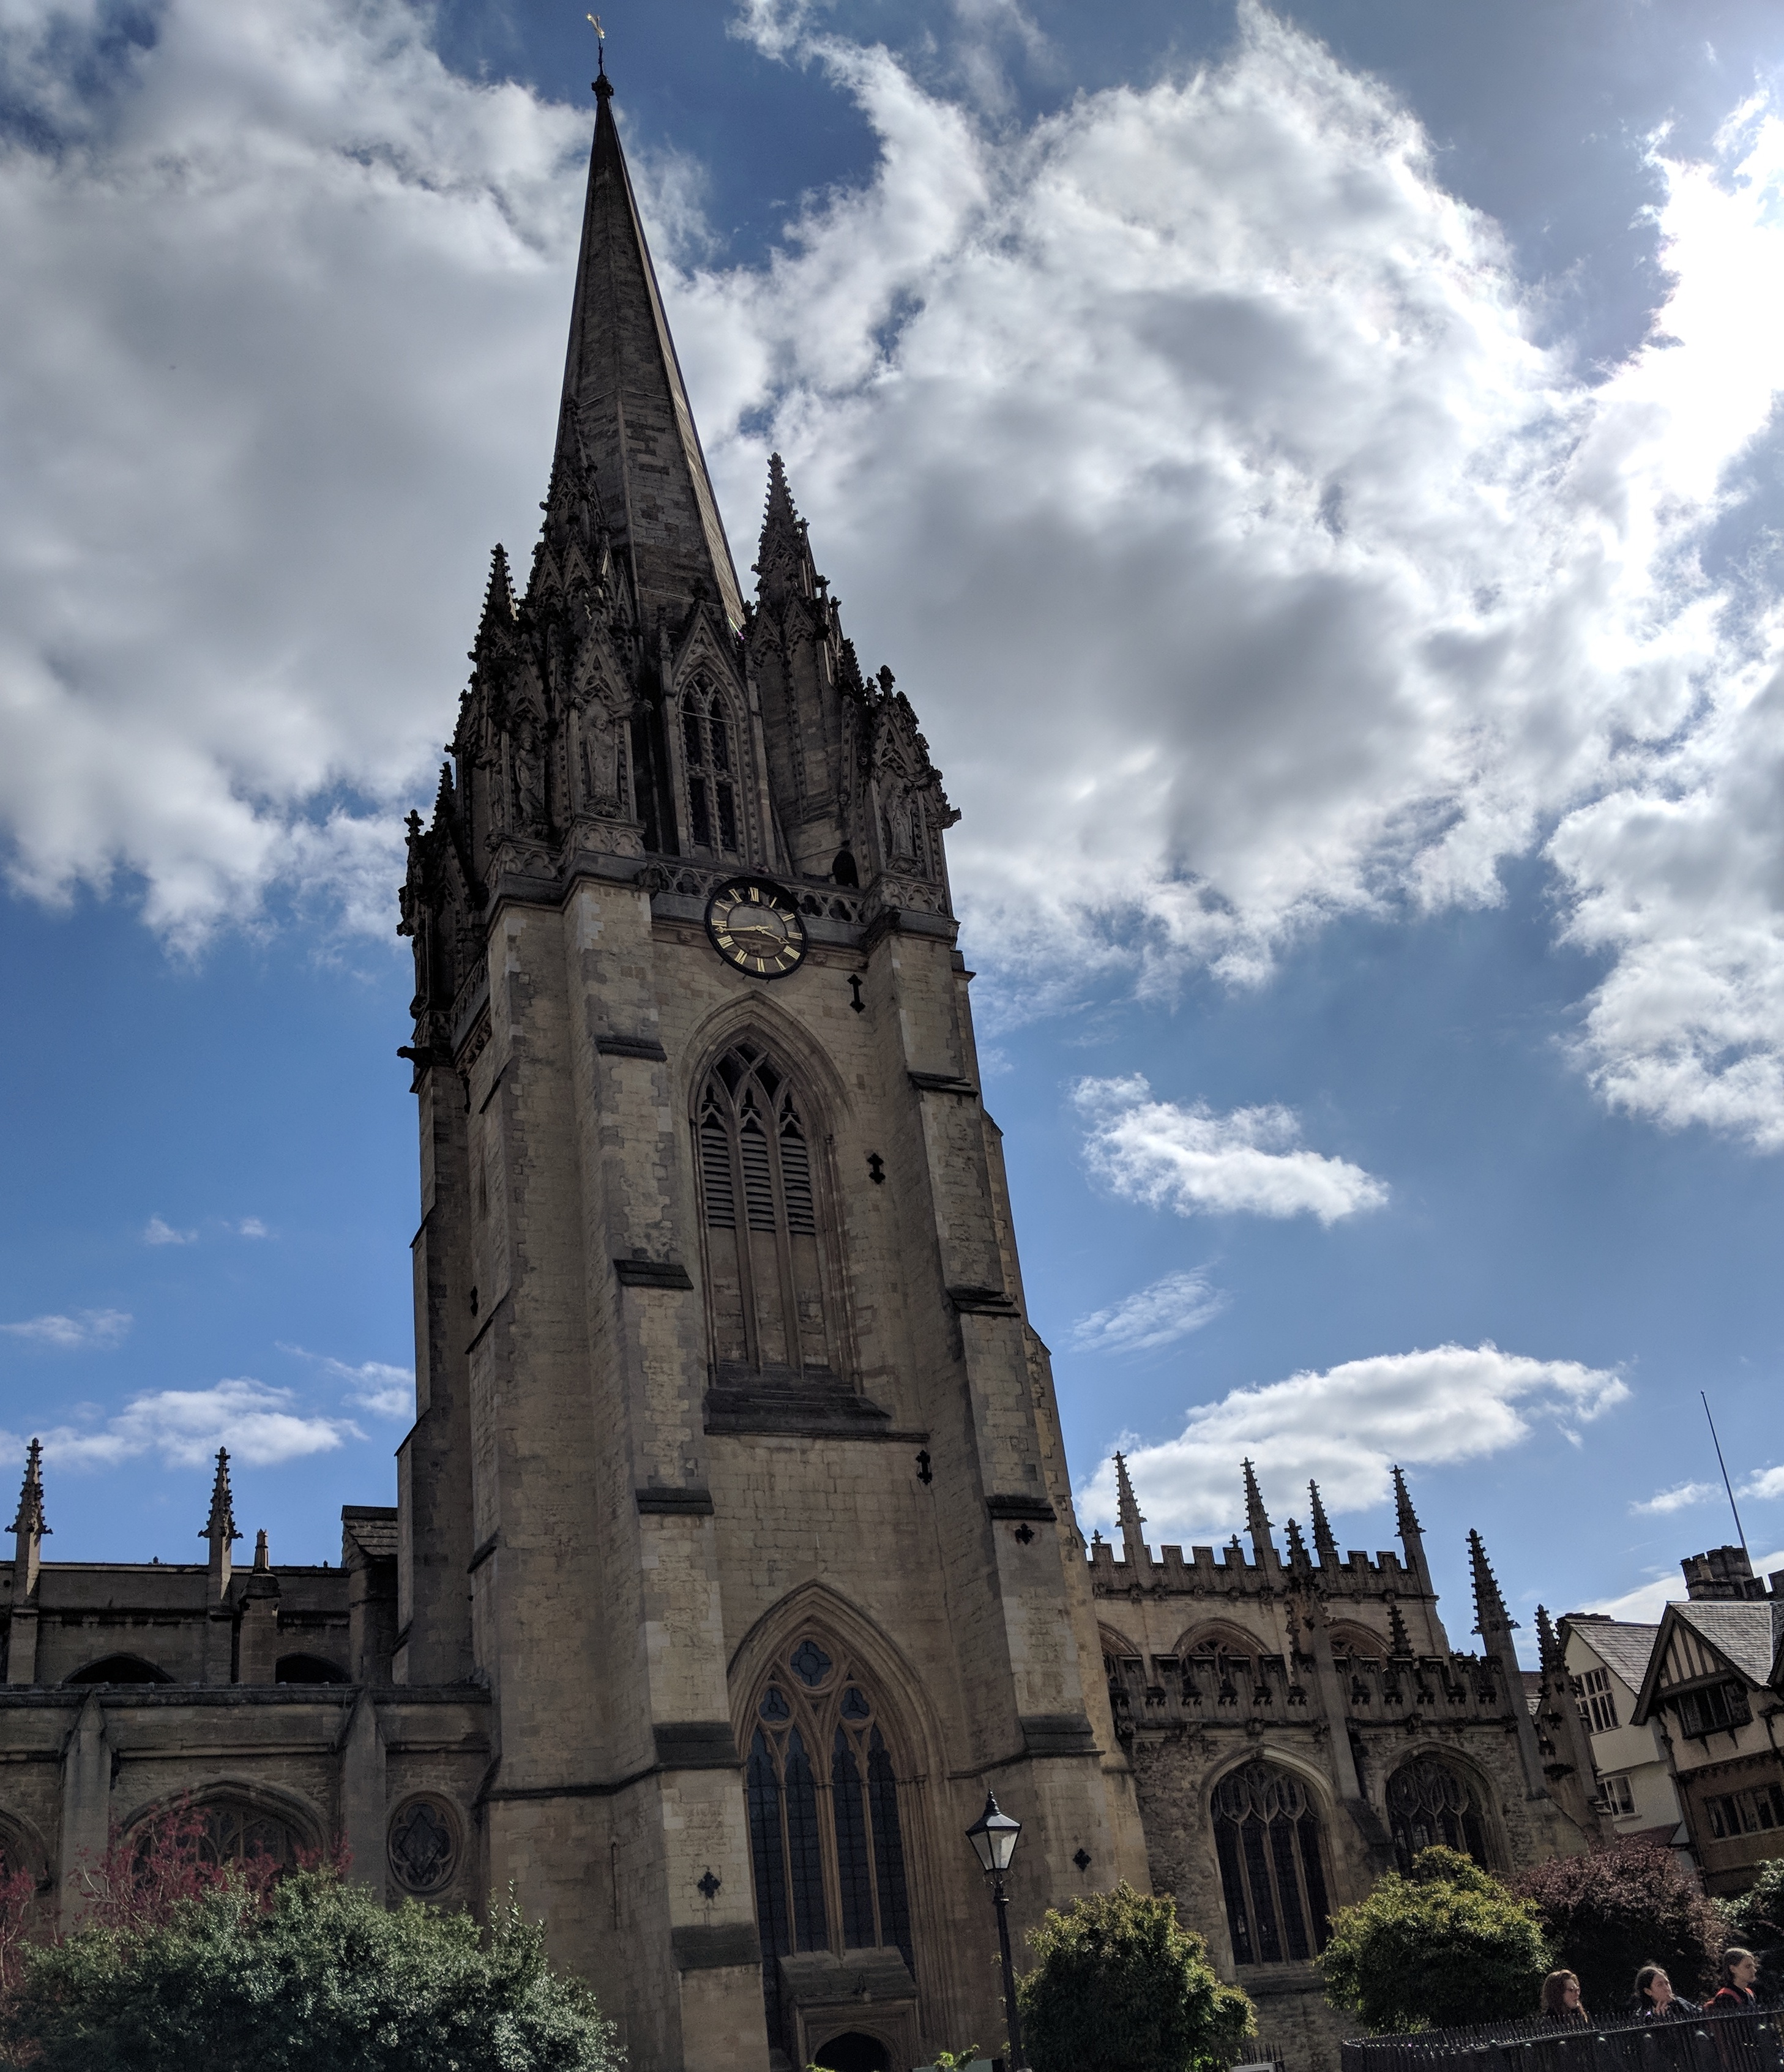
\includegraphics[height=6cm]{oxford.jpg}};
\end{tikzpicture}
\end{frame}

\begin{frame}
\begin{columns}
\begin{column}{0.45\textwidth}
{\LARGE Quantum Bernoulli Factory}
\end{column}
\begin{column}{0.25\textwidth}
\centering
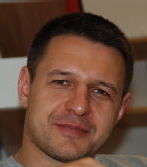
\includegraphics[width=\textwidth]{krys.jpg}\\
Krys \L atuszynski
\end{column}
\begin{column}{0.25\textwidth}
\centering
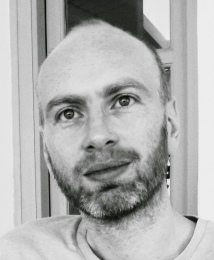
\includegraphics[width=\textwidth]{jennings.jpg}\\
David Jennings\\
(Imperial)
\end{column}
\end{columns}
\end{frame}


\begin{frame}
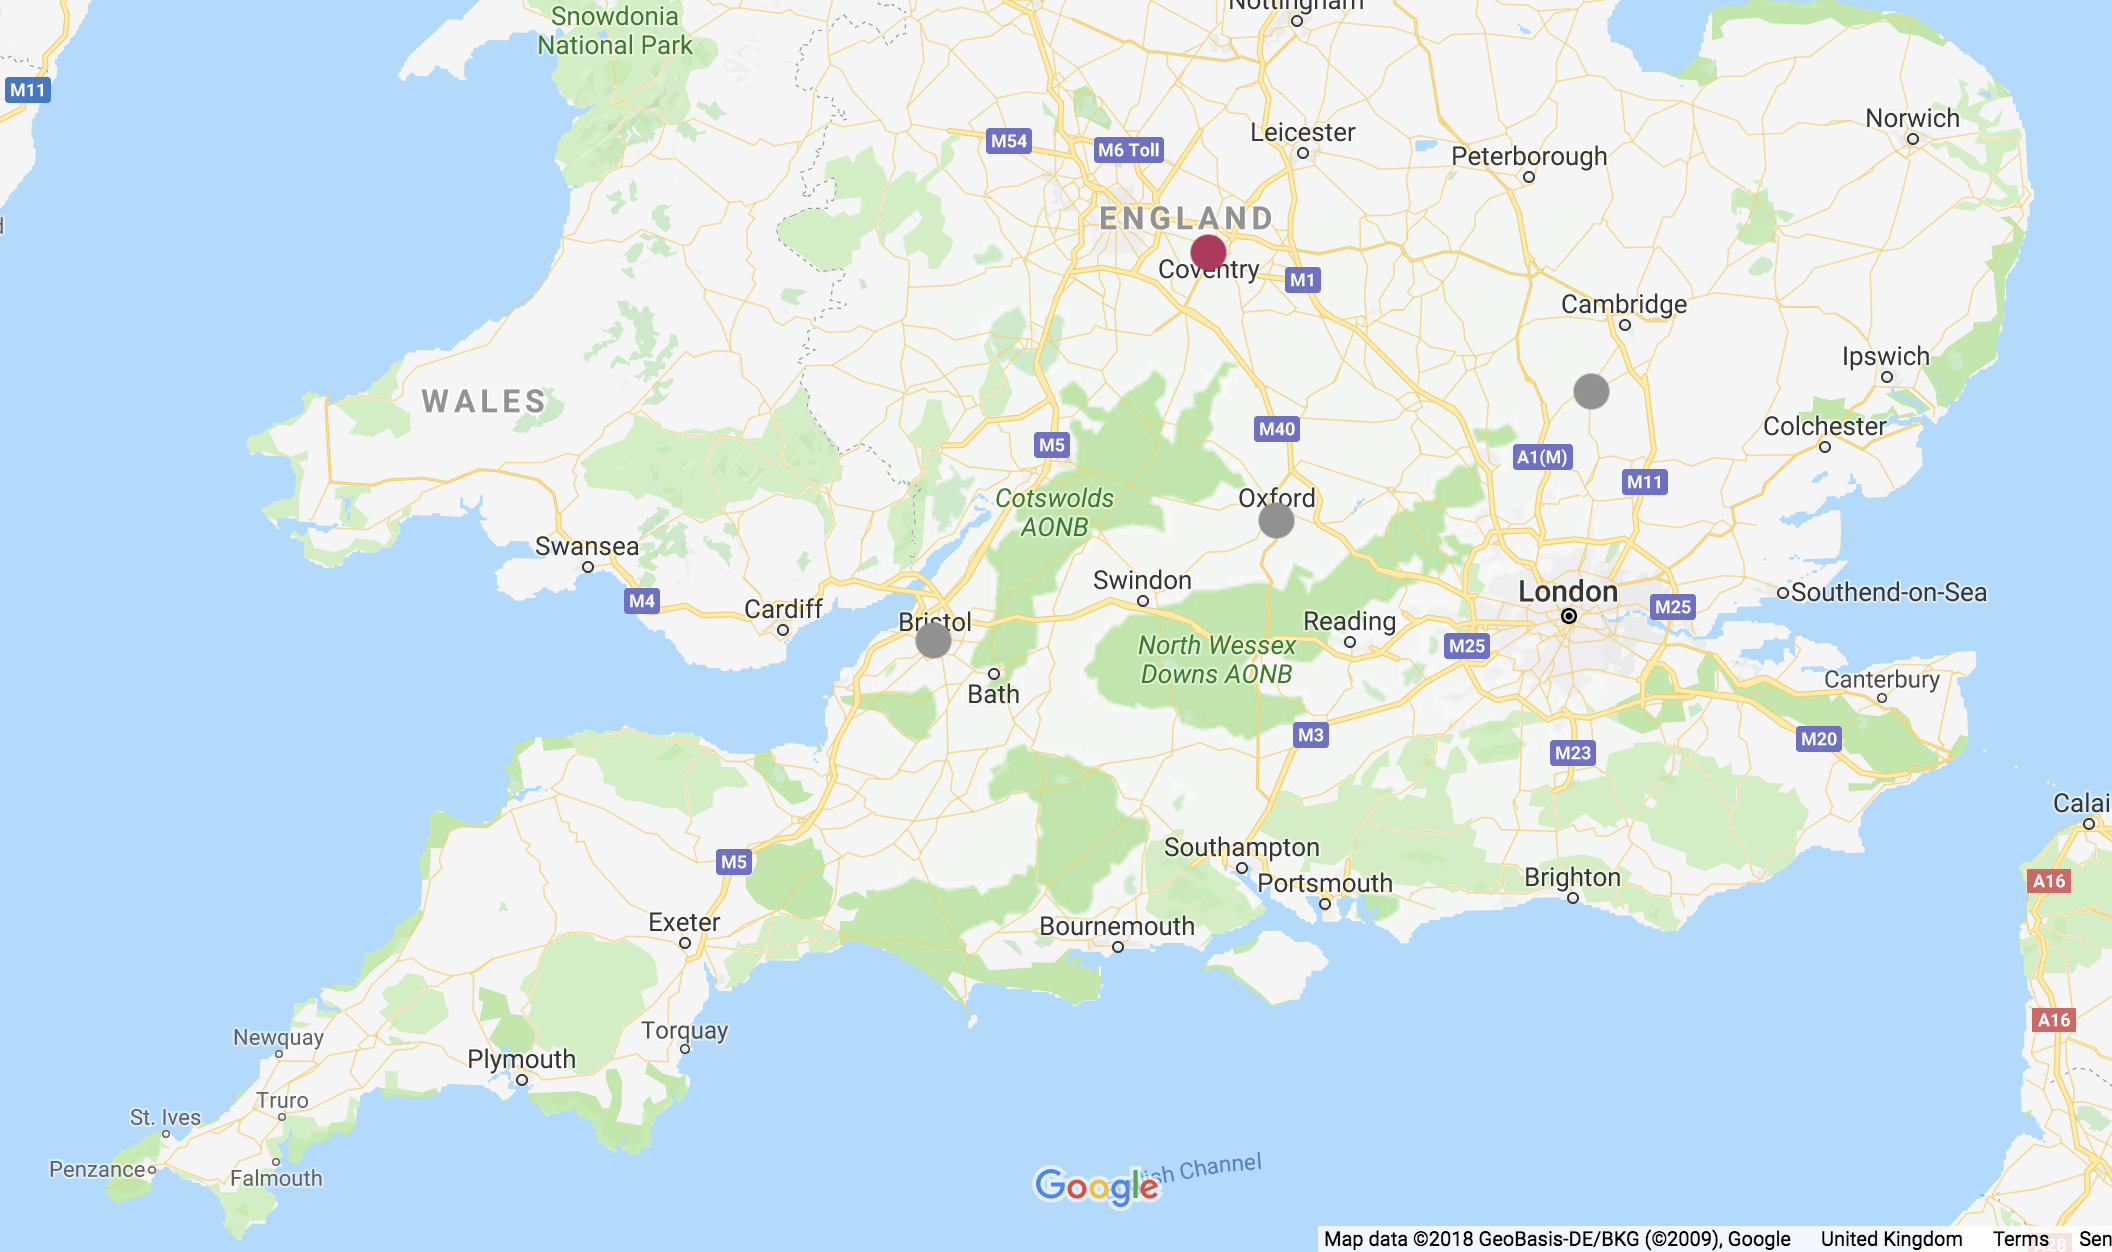
\includegraphics[width=\textwidth]{map4.png}
\end{frame}

\begin{frame}
\begin{columns}
\begin{column}{0.4\textwidth}
{\LARGE Genealogies of Sequential Monte Carlo Algorithms}
\end{column}
\begin{column}{0.2\textwidth}
\centering
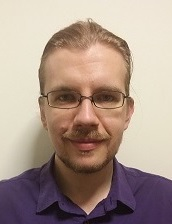
\includegraphics[width=\textwidth]{jere.jpg}\\
Jere Koskela
\end{column}
\begin{column}{0.2\textwidth}
\centering
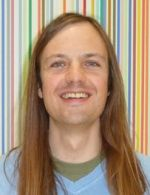
\includegraphics[width=\textwidth]{adam.jpg}\\
Adam Johansen
\end{column}
\begin{column}{0.2\textwidth}
\centering
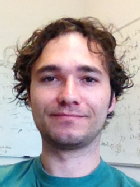
\includegraphics[width=\textwidth]{paul.png}\\
Paul Jenkins
\end{column}
\end{columns}
\end{frame}

\begin{frame}
\end{frame}

\end{document}